%-------------------------------
%	DOCUMENT SETTINGS
%-------------------------------
\documentclass[a4paper]{article}

\setlength{\hoffset}{-3.2cm}
\setlength{\voffset}{-3cm}
\setlength{\textwidth}{18.7cm}
\setlength{\textheight}{25.5cm}
\setlength{\parskip}{0pt}
\setlength{\parindent}{0in}

%----------------------------------------------------------------------------------------
%	PACKAGES AND OTHER DOCUMENT CONFIGURATIONS
%----------------------------------------------------------------------------------------

\usepackage{mathtools}
\usepackage[table]{xcolor} % Driver-independent color extensions, para table-generators
\usepackage[utf8]{inputenc} % Use UTF-8 encoding
\usepackage{microtype} % Slightly tweak font spacing for aesthetics
\usepackage[english]{babel} % Language hyphenation and typographical rules
\usepackage{amsthm, amsmath, amssymb} % Mathematical typesetting
\usepackage{float} % Improved interface for floating objects
\usepackage[final, colorlinks = true, linkcolor = black, citecolor = black]{hyperref} % For hyperlinks in the PDF
\usepackage{dsfont}
\DeclarePairedDelimiter\abs{\lvert}{\rvert}%
\usepackage{cancel}
\usepackage{charter} % Use the Charter font
\usepackage{graphicx, multicol} % Enhanced support for graphics
\usepackage{booktabs} % Enhances quality of tables
\usepackage{tikz-qtree} % Easy tree drawing tool
% Configuration for b-trees and b+-trees, !uses style file!
%\usepackage[backend=biber,style=numeric,
%            sorting=nyt]{biblatex} % Complete reimplementation of bibliographic facilities
%\addbibresource{ecl.bib}

\usepackage[yyyymmdd]{datetime} % Uses YEAR-MONTH-DAY format for dates
\renewcommand{\dateseparator}{-} % Sets dateseparator to '-'
\usepackage{fancyhdr} % Headers and footers

\pagestyle{fancy} % All pages have headers and footers
\fancyhead{}\renewcommand{\headrulewidth}{0pt} % Blank out the default header
\fancyfoot[L]{} % Custom footer text
\fancyfoot[C]{} % Custom footer text
\fancyfoot[R]{\thepage} % Custom footer text
\newcommand{\note}[1]{\marginpar{\scriptsize \textcolor{red}{#1}}} % Enables comments in red on margin

%----------------------------------------------------------------------------------------
%	CUSTOM COMMANDS
%----------------------------------------------------------------------------------------

\newcommand{\R}{\mathbb{R}}
\newcommand{\E}{\mathbb{E}}
\newcommand{\I}{\mathbb{I}}
\newcommand{\Var}{\text{Var}}
% Para poner sonrisa sobre puntos suspensivos. Uso: \overplace{n}{\dotsc}
\newcommand{\overplace}[2]{%
	\overset{\substack{#1\\\smile}}{#2}%
}

\begin{document}

%-------------------------------
%	TITLE SECTION
%-------------------------------

\fancyhead[C]{}
\hrule \medskip % Upper rule
\begin{minipage}{0.295\textwidth} 
	\raggedright
	\footnotesize
	José Antonio Álvarez Ocete \hfill\\   
	Francisco Javier Sáez Maldonado \hfill
\end{minipage}
\begin{minipage}{0.4\textwidth} 
	\centering 
	\large 
	Exploración Gráfica de Datos \\ 
	\normalsize 
	Gestión de Datos \\ 
\end{minipage}
\begin{minipage}{0.295\textwidth} 
	\raggedleft
	\today\hfill\\
\end{minipage}
\medskip\hrule 
\bigskip

%-------------------------------
%	CONTENTS
%-------------------------------

\section{Objetivos}

En esta práctica estudiaremos un dataset de \emph{CardSorting} para ver las relaciones entre diversos productos de supermercado. Para ello emplearemos diferentes técnicas de visualización de datos como: un hisograma, un \emph{heatmap}, un dendograma y un grafo de similitudes entre tarjetas.

\section{Lectura y limpieza de datos}

En primer lugar, utilizamos las funciones \emph{read.csv} y \emph{url} de R para leer los datos del dataset utilizando la dirección \url{http://cardsorting.net/tutorials/25.csv}. Como únicamente estamos interesados en los datos numéricos, eliminamos las columnas \emph{Uniqid}, \emph{Category}, \emph{Startdate}, \emph{Starttime}, \emph{Endtime}, \emph{QID} y \emph{Comments}.

\section{Densidad númerica de los datos}

Como primera aproximación a la visualización de estos datos estamos interesados en conocer los valores númericos que toma nuestro dataset, así como la distribución entre los mismos. Para ello nuestra mejor herramienta será un simple histograma sobre el dataset completo.

\begin{figure}[H]
	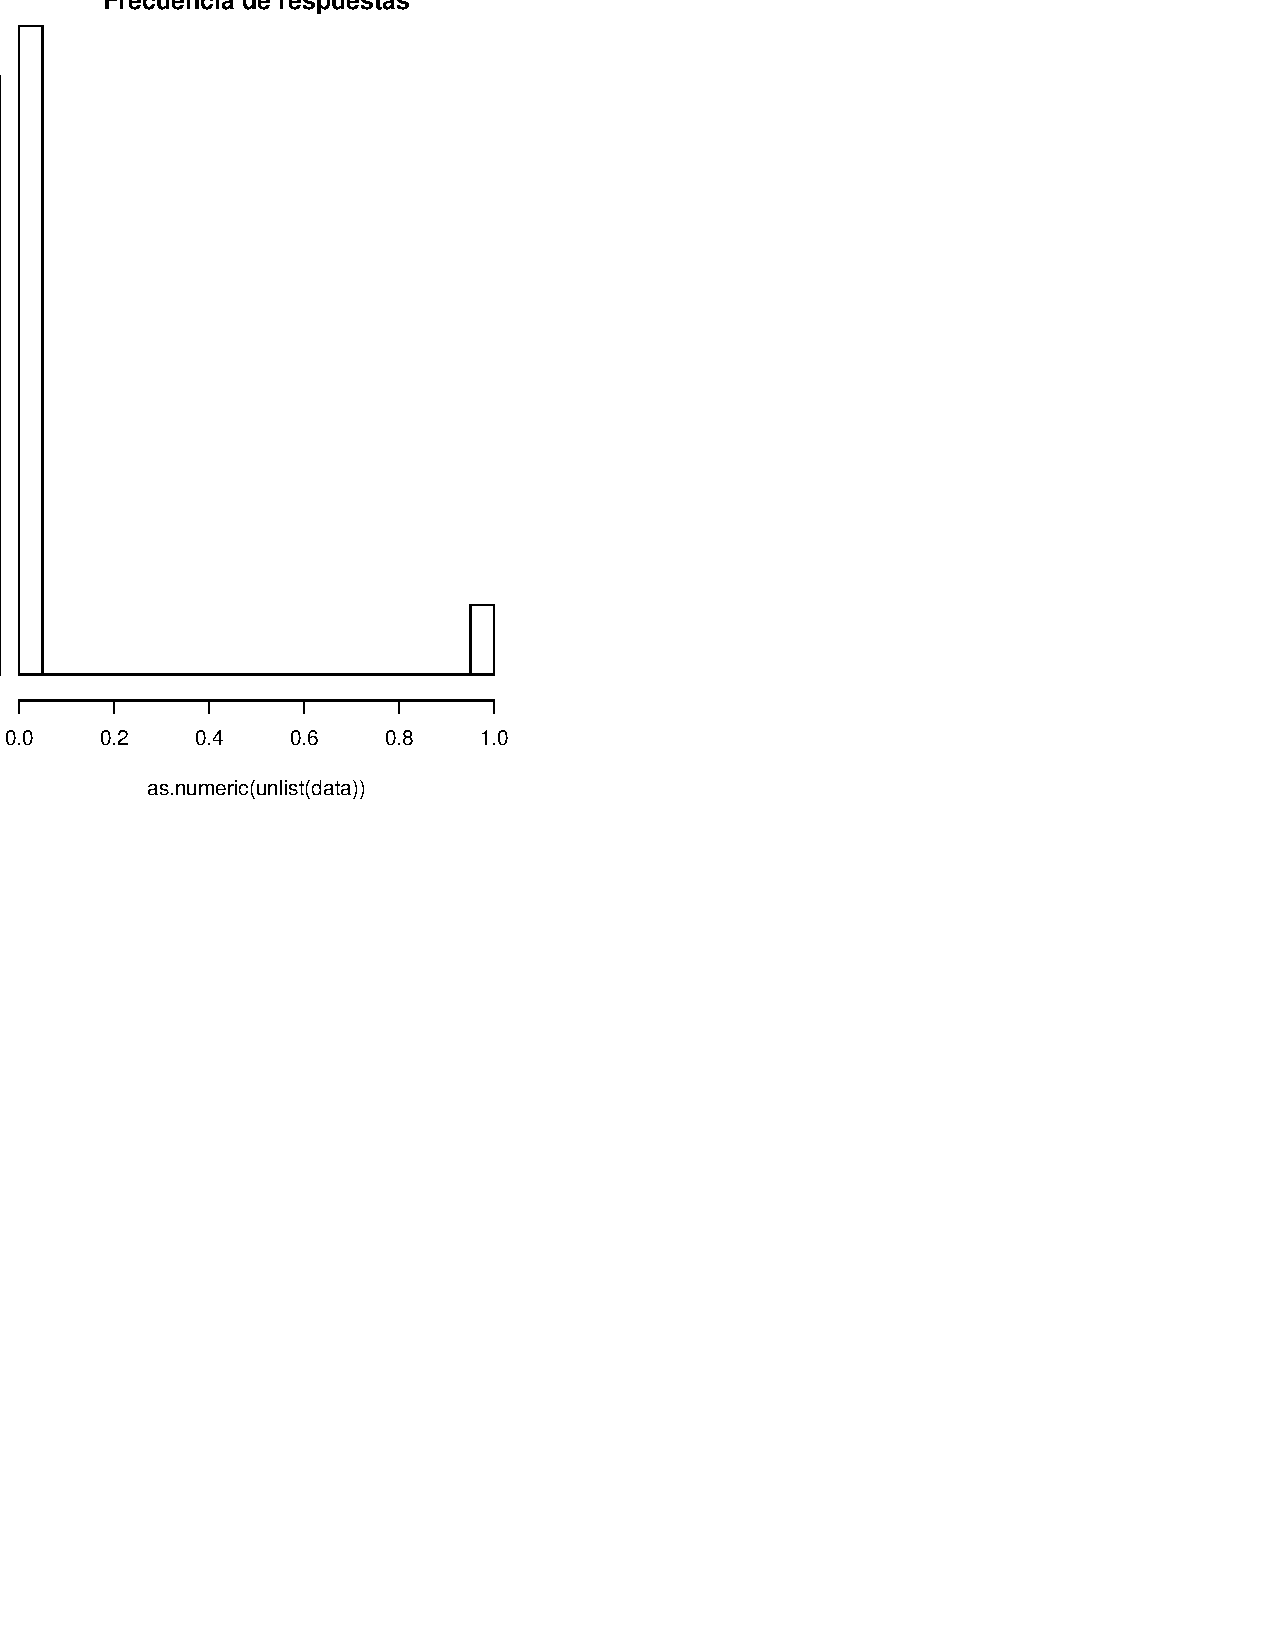
\includegraphics[scale=.6]{figures/hist}
	\centering
	\caption{Histograma de nuestro dataset.}
\end{figure}

Vemos como la mayoría de los valores están en $0$, mientras que algunos pocos toman el valor $1$. Recordemos la información que codifica este dataset: cada columna es un producto del supermercado (una \emph{card} en nuestro \emph{CardSorting}), mientras que cada fila es una categoría, introducida por el usuario con Id asociado \emph{Uniqid}. Un $1$ significa que el usuario ha asociado ese producto con esa categoría, y un $0$ que no lo ha hecho. \\

Por un lado, nuestro análisis númerico dado por el histograma encaja con nuestra intuición: la gran mayoría de los valores serán $0$. Por otro lado, puesto que las categorías son introducidas por los usuarios de forma manual, obtendremos muchas categorías similiares pero ligeramente distintas. Por ejemplo, para frutas y verduras obtenemos entre otras las siguientes categorías: \emph{fruits}, \emph{veggies}, \emph{fruits and veggies} y \emph{frutis and veggies}.

\section{Similitud entre tarjetas}

Tras una primera impresión de la distribución numérica de los datos, procedemos a realizar un estudio sobre la similitud hayada entre las tarjetas de este dataset. Para ello computaremos la matriz de distancias entre las distintas tarjetas, utilizando la distancia euclídea. Cabe destacar que puesto que los valores de nuestro dataset están en $\{0,1\}$, $x^2 = x$, y la distancia en $L_1$ será equivalente a la distancia euclídea de $L_2$. A pesar de ello, sería interesante utilizar distintas distancias para comparar los resultados entre ambas. \\

Tras computar la matriz de distancias hacemos uso de la función \emph{heatmap.2} de R para representar un mapa de calor. Valores más bajos (rojos) representarán distancias más bajas. Es decir, tarjetas más relacionadas. En contraparte, valores más altos (amarillo claro y blanco) representarán distancias altas. Es decir, tarjetas poco relacionadas. \\

\begin{figure}[H]
	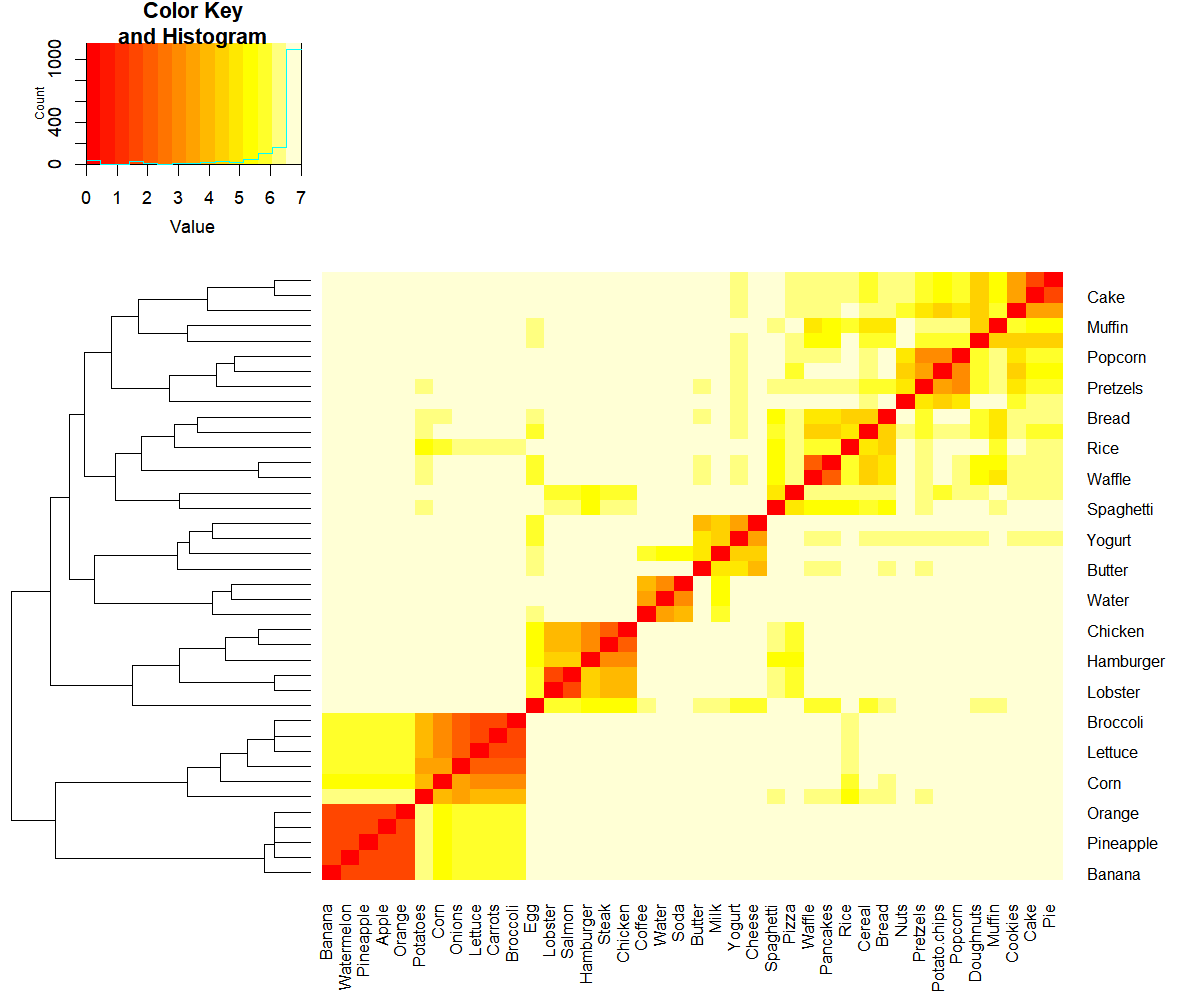
\includegraphics[scale=.6]{figures/heatmap}
	\centering
	\caption{Heatmap y dendograma de las distancias entre tarjetas.}
\end{figure}

Vemos un bloque de tarjetas muy relacionado entre si en la parte inferior izquierda que corresponde a las frutas, y uno cercano también muy relacionado que corresponde a las verduras: \emph{Banana}, \emph{Watermelon}, \emph{Pineapple}, \emph{Apple}, \emph{Orange}, \emph{Potatoes}, \emph{Lettuce}, \emph{Carrots} y \emph{Broccoli}. \\

Vemos también un conjunto de tarjetas relacionadas en la esquina superior derecha. Destaca en particular \emph{Pie} y \emph{Cake}. Finalmente, en la zona central pegada a las verduras hay otra pareja que destaca: \emph{Salmon} y \emph{Lobster}. Todo este tipo de relaciones tienen sentido semántica y culturalmente, lo que revela que nuestro análisis sobre la relación entre tarjetas está siendo acertado. \\

A la izquierda del \emph{heatmap} podemos ver un dendograma con las diviones en clusters y subclusters. Esto nos indica lo cercanos que están los elementos entre si de forma visualmente distintas, pero las conclusiones que podemos obtener al respecto son equivalentes a las ya comentadas. \\

\section{Relaciones entre tarjetas}

De cara a visualizar las relaciones entre tarjetas de forma aún más directa podemos utilizar un grafo ponderado, donde los nodos representarán tarjetas y los lados, las relaciones entre las mismas. Grafos más resaltados (con mayor ponderación) revelarán una mayor relación entre las tarjetas. \\

Para computar este tipo de gráfico necesitamos una matriz de similitudes en vez de una matriz de distancias como la que hemos utilizado hasta ahora. Podemos utilizar directamente la inversa elemento a elemento de esta matriz: definiremos la similitud entre dos elementos como el inverso de su distancia:

\[
	\text{Sim}(a,b) = \frac{1}{\text{dist}(a,b)}
\]

Obtenemos el siguiente gráfico como resultado:

\begin{figure}[H]
	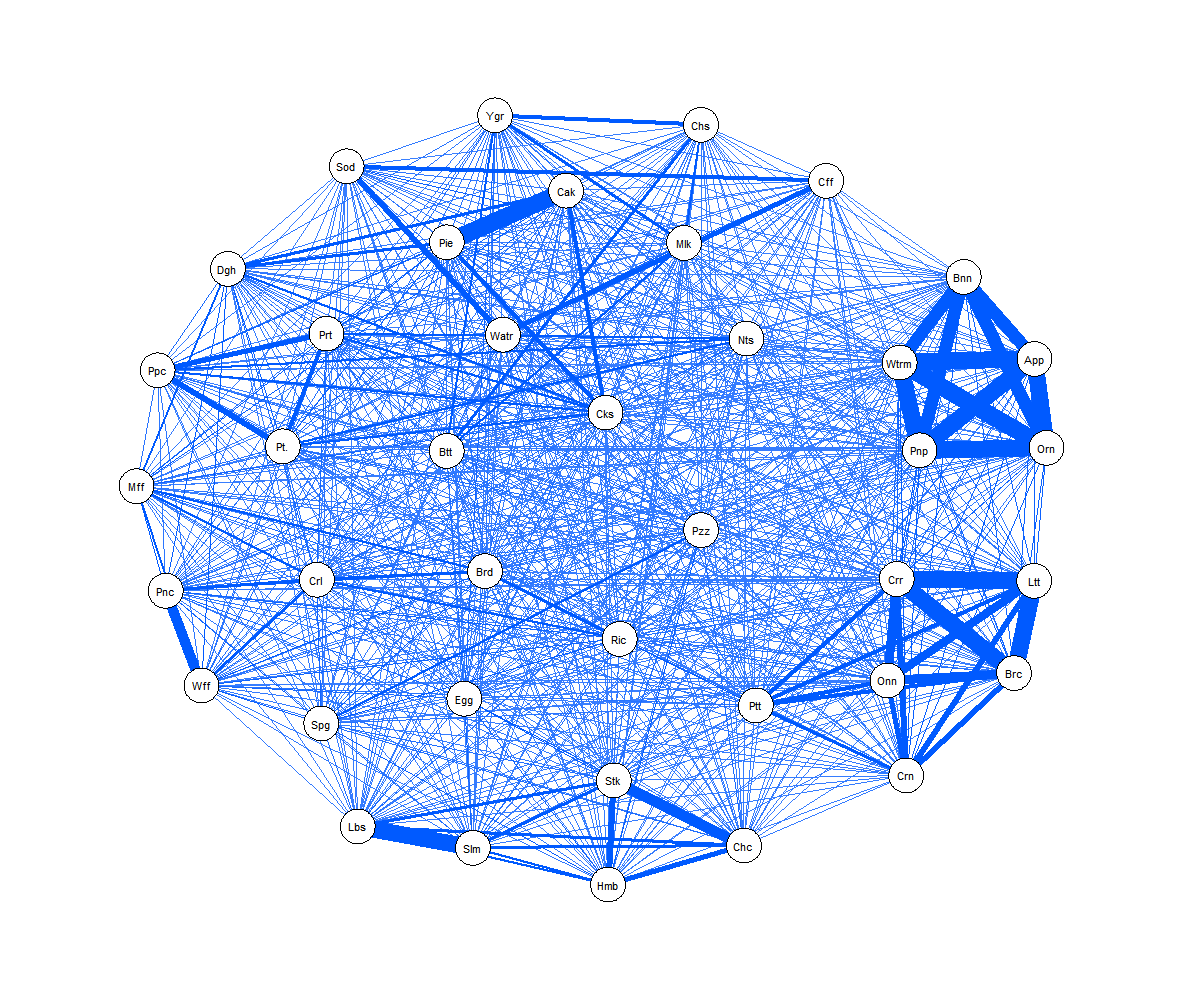
\includegraphics[scale=.6]{figures/dist}
	\centering
	\caption{Grafo ponderado de las similitud entre tarjetas}
\end{figure}

En este nuevo gráfico es sencillo apreciar los mismos resultados que en el \emph{heatmap} y en el dendograma: hay dos clusteres de elementos relacionados claramente, las frutas y las verduras, ligeramente serarados. Por otro lado encontramos fuertes relaciones entre las parejas (\emph{Salmon}, \emph{Lobster}) (\emph{Pie}, \emph{Cake}).

\section{Tarjetas más relacionadas}

Aunque hemos ido comentando este concepto a lo largo de toda la práctica podemos realizar una análisis numérico para verificar que los valores observados en los gráficos están asociados a las mayores similitudes, y verificar cuáles están cercanos pero no llegan a ser exactamente las más relacionadas entre las anteriormente mencionadas. Para ello, computamos la mínima distincia en la matriz de distancias, obteniendo $1.4142 \approx \sqrt{2}$. Es decir, las tarjetas más relacionadas se diferencian en únicamente dos valores. \\

Finalmente, mostramos una tabla con todas las parejas que alcanzan esta distancia mínima en nuestra matriz:

\begin{table}[H]
	\centering
	\begin{tabular}{
			>{\columncolor[HTML]{FFFFFF}}c 
			>{\columncolor[HTML]{FFFFFF}}c }\\
		\textbf{Item 1} & \textbf{Item 2} \\ \hline
		Broccoli        & Carrots         \\
		Lettuce         & Carrots         \\
		Orange          & Apple           \\
		Pineapple       & Apple           \\
		Watermelon      & Apple           \\
		Carrots         & Broccoli        \\
		Lettuce         & Broccoli        \\
		Pie             & Cake            \\
		Carrots         & Lettuce         \\
		Broccoli        & Lettuce         \\
		Salmon          & Lobster         \\
		Apple           & Orange          \\
		Pineapple       & Orange          \\
		Watermelon      & Orange          \\
		Cake            & Pie             \\
		Apple           & Pineapple       \\
		Orange          & Pineapple       \\
		Watermelon      & Pineapple       \\
		Lobster         & Salmon          \\
		Apple           & Watermelon      \\
		Orange          & Watermelon      \\
		Pineapple       & Watermelon     
	\end{tabular}
\end{table}

En esta tabla observamos las tarjetas previamente comentadas. En particular, las parejas (\emph{Salmon}, \emph{Lobster}) (\emph{Pie}, \emph{Cake}) están presentes, así como la mayoría de frutas y verduras. Si nos fijamos con atención podemos apreciar como \emph{Onion} no está presente en esta tabla, pues no está tan íntimamente relacionada con el resto de verduras.

\end{document}
